\section{Experimentation}
\label{sec:experimentation}

Semi-autonomous systems explore efficient policy execution involving the optimal transfer of control between human and agent. Our focus is on semi-autonomous driving, namely the optimal policy to adapt to a human's level of fatigue.

The LMDP consists of states formed by a 4-tuple: current intersection, previous intersection, driver tired (true/false), and autonomy (enabled/disabled). Actions are taken at intersections, as found in path planning in graphs (e.g., GPS). Due to real world limitations, autonomy can only be enabled on main roads and highways; in our case, this means a speed limit greater than or equal to 30 miles per hour.

% TODO: Cite UMass M.Eng. lab's paper.

Actions are simply which road to take at each intersection and, if the road allows, whether or not to enable autonomy. We aim to follow the extensive body of engineering and psychological research on driver fatigue~\cite{Ji04-RealTimeMonitoringDriverFatigue}. As such, the stochasticity within state transitions considers the probability that the driver moves from awake to tired, with a probability of 0.9.

There are two reward functions: time and autonomy. The time reward (cost) is proportional to the time spent on the road (in seconds), plus a small constant expected value of 5 (seconds) to model time spent at a traffic light, slowing down turning, or waiting for others. The autonomy reward (cost) is proportional to the time spent on the road, but is only applied if the driver is tired; otherwise, there is an epsilon penalty. For both rewards, the goal state is an absorbing state which awards zero.

It is natural to define the problem in terms of strictly optimizing time when the driver is awake, and strictly optimizing autonomy when the driver is tired. We also allow for a 10 second slack in the expected time to reach the goal (i.e., time reward), in order to favor the ease of autonomy if available.

Figure~\ref{fig:example_policy} shows an example optimal policy returned by LVI for a few roads north of Boston Commons. Each road at an intersection has an action, denoted by the arrows. Green arrows denote that autonomy was disabled; purple arrows denote that autonomy was enabled. The blue colored roads show autonomy-capability. % TODO: Explain image in Discussion.

\begin{figure}% [H]
\begin{center}
    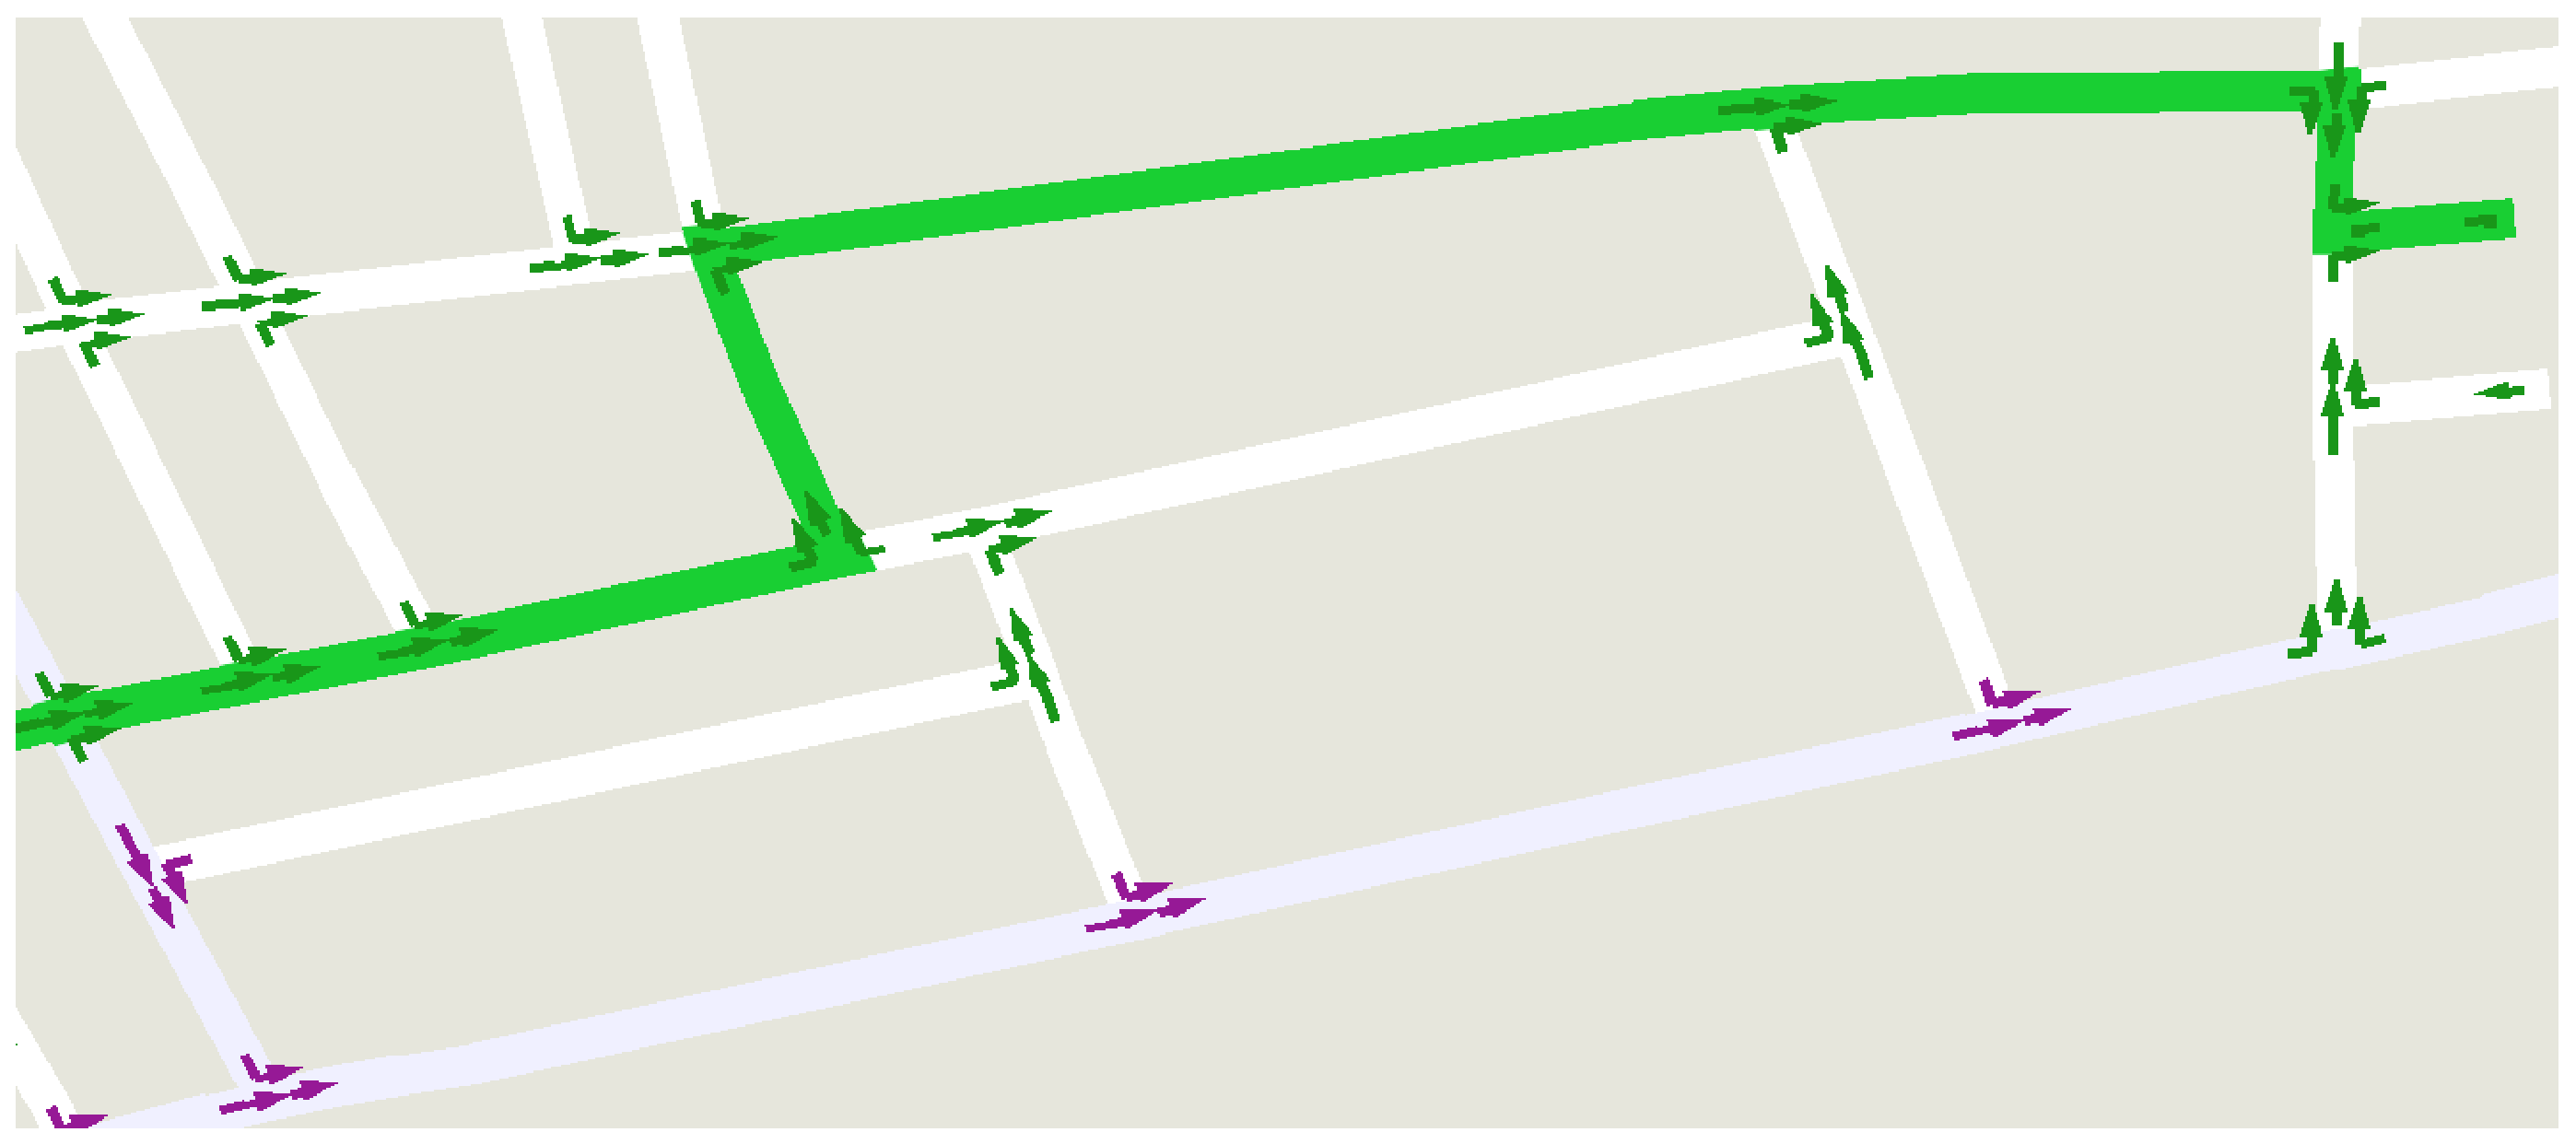
\includegraphics[width=0.75\linewidth]{awake.eps} \\
    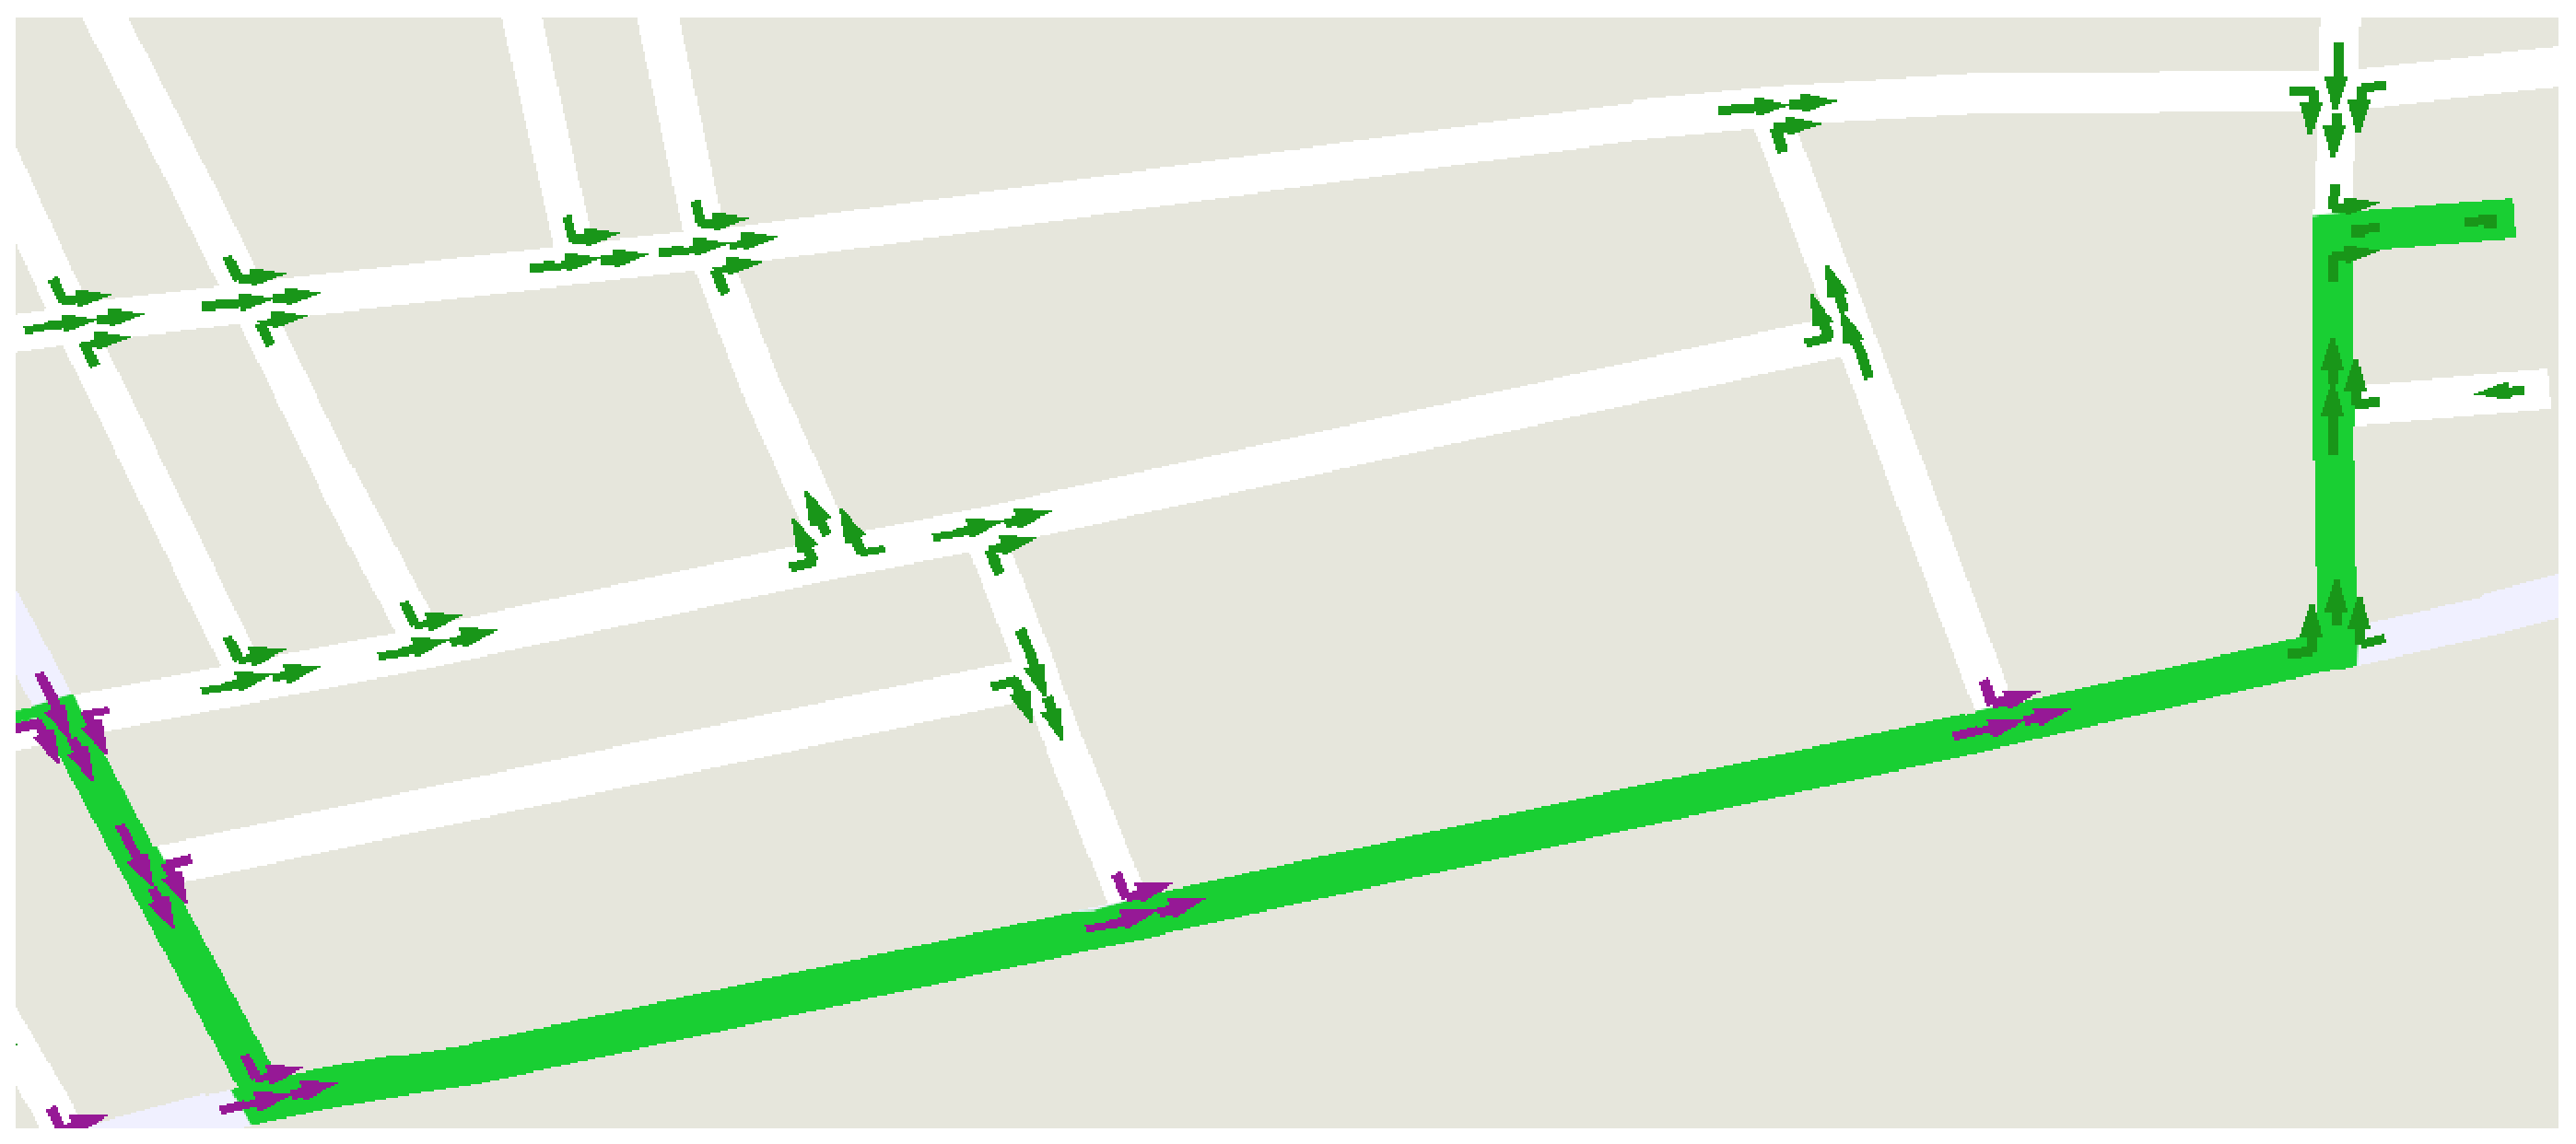
\includegraphics[width=0.75\linewidth]{tired.eps}
    \caption{The policy for awake (above) versus tired (below).}
    \label{fig:example_policy}
\end{center}
\end{figure}

% TODO: Include table for multiple cities, say 5, with state space size |S|, action size |A|, and the times for CPU vs CUDA (possibly varying blocks and threads). Compare with VI under fixed weights.

% TODO: Describe the CUDA implementation of LVI.

% TODO: State machine specs.

